\section{Methods} \label{methods}

\subsection{Study population}
This study analyzed data from the Hamburg City Health Study (HCHS), an ongoing prospective, population-based cohort study aiming to recruit a cross-sectional sample of \num{45000} adult participants from the city of Hamburg, Germany \citep{Jagodzinski2020-lx}.
From the first \num{10000} participants of the HCHS, we planned to include those who were documented to have received brain imaging (n=2648) and exclude those who were analyzed in our previous report \citep{Schlemm2022-he} (n=970).
The ethical review board of the Landesärztekammer Hamburg (State of Hamburg Chamber of Medical Practitioners) approved the HCHS (PV5131), and all participants provided written informed consent.

\subsection{Demographic and clinical characterization}
From the study database, we extracted the participants’ age at the time of inclusion in years, their sex, and the number of years spent in education.
During the visit to the study center, participants underwent cognitive assessment using standardized tests.
From the database, we extracted their performance scores on the Trail Making Test part B, measured in seconds, as an operationalization of executive function and psychomotor processing speed \citep{Tombaugh2004-dp,arbuthnott2000trail}.
For descriptive purposes, we also extracted data on past medical history and reported the proportion of participants with a previous diagnosis of dementia.

\subsection{MRI acquisition and preprocessing}
The magnetic resonance imaging protocol for the HCHS includes structural and resting-state functional sequences.
The acquisition parameters for a \qty{3}{\tesla} Siemens Skyra MRI scanner (Siemens, Erlangen, Germany) have been previously reported \citep{Petersen2020-cx,Frey2021-sv} and are given as follows:

For $T_1$-weighted anatomical images, a 3D rapid acquisition gradient-echo sequence (MPRAGE) was used with the following sequence parameters: repetition time $\text{TR} = \qty{2500}{\ms}$, echo time $\text{TE} = \qty{2.12}{\ms}$, 256 axial slices, slice thickness $\text{ST} = \qty{0.94}{\mm}$, and in-plane resolution  $\text{IPR} = \qtyproduct[product-units = bracket-power]{0.83 x 0.83}{\mm}$.

$T_2$-weighted fluid attenuated inversion recovery (FLAIR) images were acquired with the following sequence parameters: $\text{TR} = \qty{4700}{\ms}$, $\text{TE} = \qty{392}{\ms}$, \num{192} axial slices, $\text{ST} = \qty{0.9}{\mm}$, $\text{IPR} = \qtyproduct[product-units = bracket-power]{0.75 x 0.75}{\mm}$.

\num{125} resting state functional MRI volumes were acquired ($\text{TR} = \qty{2500}{\ms}$; $\text{TE} = \qty{25}{\ms}$; $\text{flip angle} = \ang[]{90}$; slices = \num{49}; $\text{ST} = \qty{3}{\mm}$; $\text{slice gap} = \qty{0}{\mm}$; $\text{IPR} = \qtyproduct[product-units = bracket-power]{2.66 x 2.66}{\mm}$).
The subjects were asked to keep their eyes open and to think of nothing.

We verified the presence and voxel dimensions of expected MRI data for each participant and excluded those for whom at least one of $T_1$-weighted, FLAIR, and resting-state MRI was missing. We also excluded participants with neuroradiologically confirmed space-occupying intra-axial lesion.
To ensure reproducibility, no visual quality assessment of raw images was performed.

For the remaining participants, structural and resting-state functional MRI data was preprocessed using FreeSurfer v6.0 (\url{https://surfer.nmr.mgh.harvard.edu/}), and fmriPrep v20.2.6 \citep{Esteban2019-sx}, using default parameters. Participants were excluded if automated processing using at least one of these packages failed.

\subsection{Quantification of WMH load}
For our primary analysis, the extent of ischemic white matter disease was operationalized as the total volume of supratentorial WMHs obtained from automated segmentation using a combination of anatomical priors, BIANCA \citep{Griffanti2016-dt}, and LOCATE \citep{Sundaresan2019-ww}, post-processed with a minimum cluster size of \num{30} voxels, as described in \citep{Schlemm2022-he}.
In an exploratory analysis, we partitioned voxels identified as WMH into deep and periventricular components according to their distance to the ventricular system (cut-off $\qty{10}{\mm}$, \citep{Griffanti2018-oa})

\subsection{Brain state estimation}
The output from fMRIprep was post-processed using xcpEngine v1.2.3 to obtain de-confounded spatially averaged BOLD time series \citep{Ciric2017-cl}.
For the primary analysis, we used the \textit{36p} regression strategy and the Schaefer-\num{400} parcellation \citep{Schaefer2018-bo}, as in \citep{Schlemm2022-he}.
 
Different atlases and confound regression strategies, as implemented in xcpEngine, were included in an exploratory multiverse analysis.

Co-activation pattern (CAP) analysis was performed by first aggregating parcellated, de-confounded BOLD signals into a $\left(n_{\text{parcels}}\times \sum_i{n_{\text{time points}, i}}\right)$ feature matrix, where $n_{\text{time points}, i}$ denotes the number of retained volumes for subject $i$ after confound regression.
Clustering was performed using the $k$-means algorithm ($k=5$) with a distance measure given by 1 minus the sample Pearson correlation between points, as implemented in Matlab R2021a.
We estimated the subject- and state-specific fractional occupancies, which are defined as the proportion of BOLD volumes assigned to each brain state \citep{Vidaurre2018-pb}. 
The two states with the highest average occupancies were identified as the basis for further analysis.

\subsection{Statistical analysis}
For demographic (age, sex, and years of education) and clinical (TMT-B) variables, the number of missing items is reported.
For non-missing values, we provide descriptive summary statistics using median and interquartile range.
The proportions of men and women in the sample are reported. Since we expected based on our pilot data \citep{Schlemm2022-he} that the proportion of missing data would be small, primary regression modelling was carried out as a complete-case analysis.

As an outcome-neutral quality check of the implementation of the MRI processing pipeline, brain state estimation, and co-activation pattern analysis, we compared fractional occupancies between brain states.
We expected that the average fractional occupancy in the two high-occupancy states would be higher than the average fractional occupancy in the other three states.
Point estimates and 95\% confidence intervals are presented for the difference in average fractional occupancy to verify this assertion.

For further analyses, non-zero WMH volumes were subjected to logarithmic transformation.
Zero values retained their value of zero; to compensate, all models included a binary indicator for zero WMH volume if at least one non-zero WMH value was present.

To assess the primary hypothesis of a negative association between the extent of ischemic white matter disease and time spent in high-occupancy brain states, we performed a fixed-dispersion Beta regression to model the logit of the conditional expectation of the average fractional occupancy of two high-occupancy states as an affine function of the logarithmized WMH load.
Age and sex were included as covariates.
The strength of the association was quantified as the odds ratio per interquartile ratio of the WMH burden distribution, and is accompanied by a 95\% confidence interval.
Significance testing of the null hypothesis of no association was conducted at the conventional significance level of 0.05.
Estimation and testing were carried out using the 'betareg' package v3.1.4 in R v4.2.1.

To  assess the secondary hypothesis of an association between time spent in high-occupancy brain states and executive dysfunction, we performed a generalized linear regression with a Gamma response distribution to model the logarithm of the conditional expected completion time in part B of the TMT as an affine function of the average fractional occupancy of two high-occupancy states.
Age, sex, years of education, and logarithmized WMH load were included as covariates.
The strength of the association was quantified as a multiplicative factor per percentage point and accompanied by a 95\% confidence interval.
Significance testing of the null hypothesis of no association was conducted at the conventional significance level of 0.05.
Estimation and testing were performed using the glm function included in the 'stats' package from R v4.2.1.

\subsection{Pre-registered analyses}
The analysis plan was pre-restistered on June 27 2023 at \url{https://osf.io/fcqmb}. The sample size calculation was based on an effect size on the odds ratio scale of 0.95, corresponding to an absolute difference in the probability of occupying a DMN-related brain state between the first and third WMH-load quartile of 1.3 percentage points, and between the 5\% and 95\% percentile of 3.1 percentage points. Approximating half the difference in fractional occupancy of DMN-related states between different task demands (rest vs n-back) in healthy subjects, which was estimated to lie between 6 and 7 percentage points \citep{Cornblath2020-fu}, this value represented a plausible choice for the smallest effect size of theoretical and practical interest. It also equals the estimated effect size based on the data presented in \citep{Schlemm2022-he}.

Simple bootstrapping was used to create \num{10000} hypothetical datasets of size \num{200}, \num{400}, \num{600}, \num{800}, \num{900}, \num{910}, \ldots, \num{1090}, \num{1100}, \num{1200}, \num{1400}, \num{1500}, and \num{1600}.
Each dataset was then subjected to the estimation procedure described above.
For each sample size, the proportion of datasets in which the primary null hypothesis of no association between fractional occupancy and WMH load could be rejected at $\alpha=0.05$ was computed and recorded as a power curve in \Cref{fig:power}.

\begin{figure}
    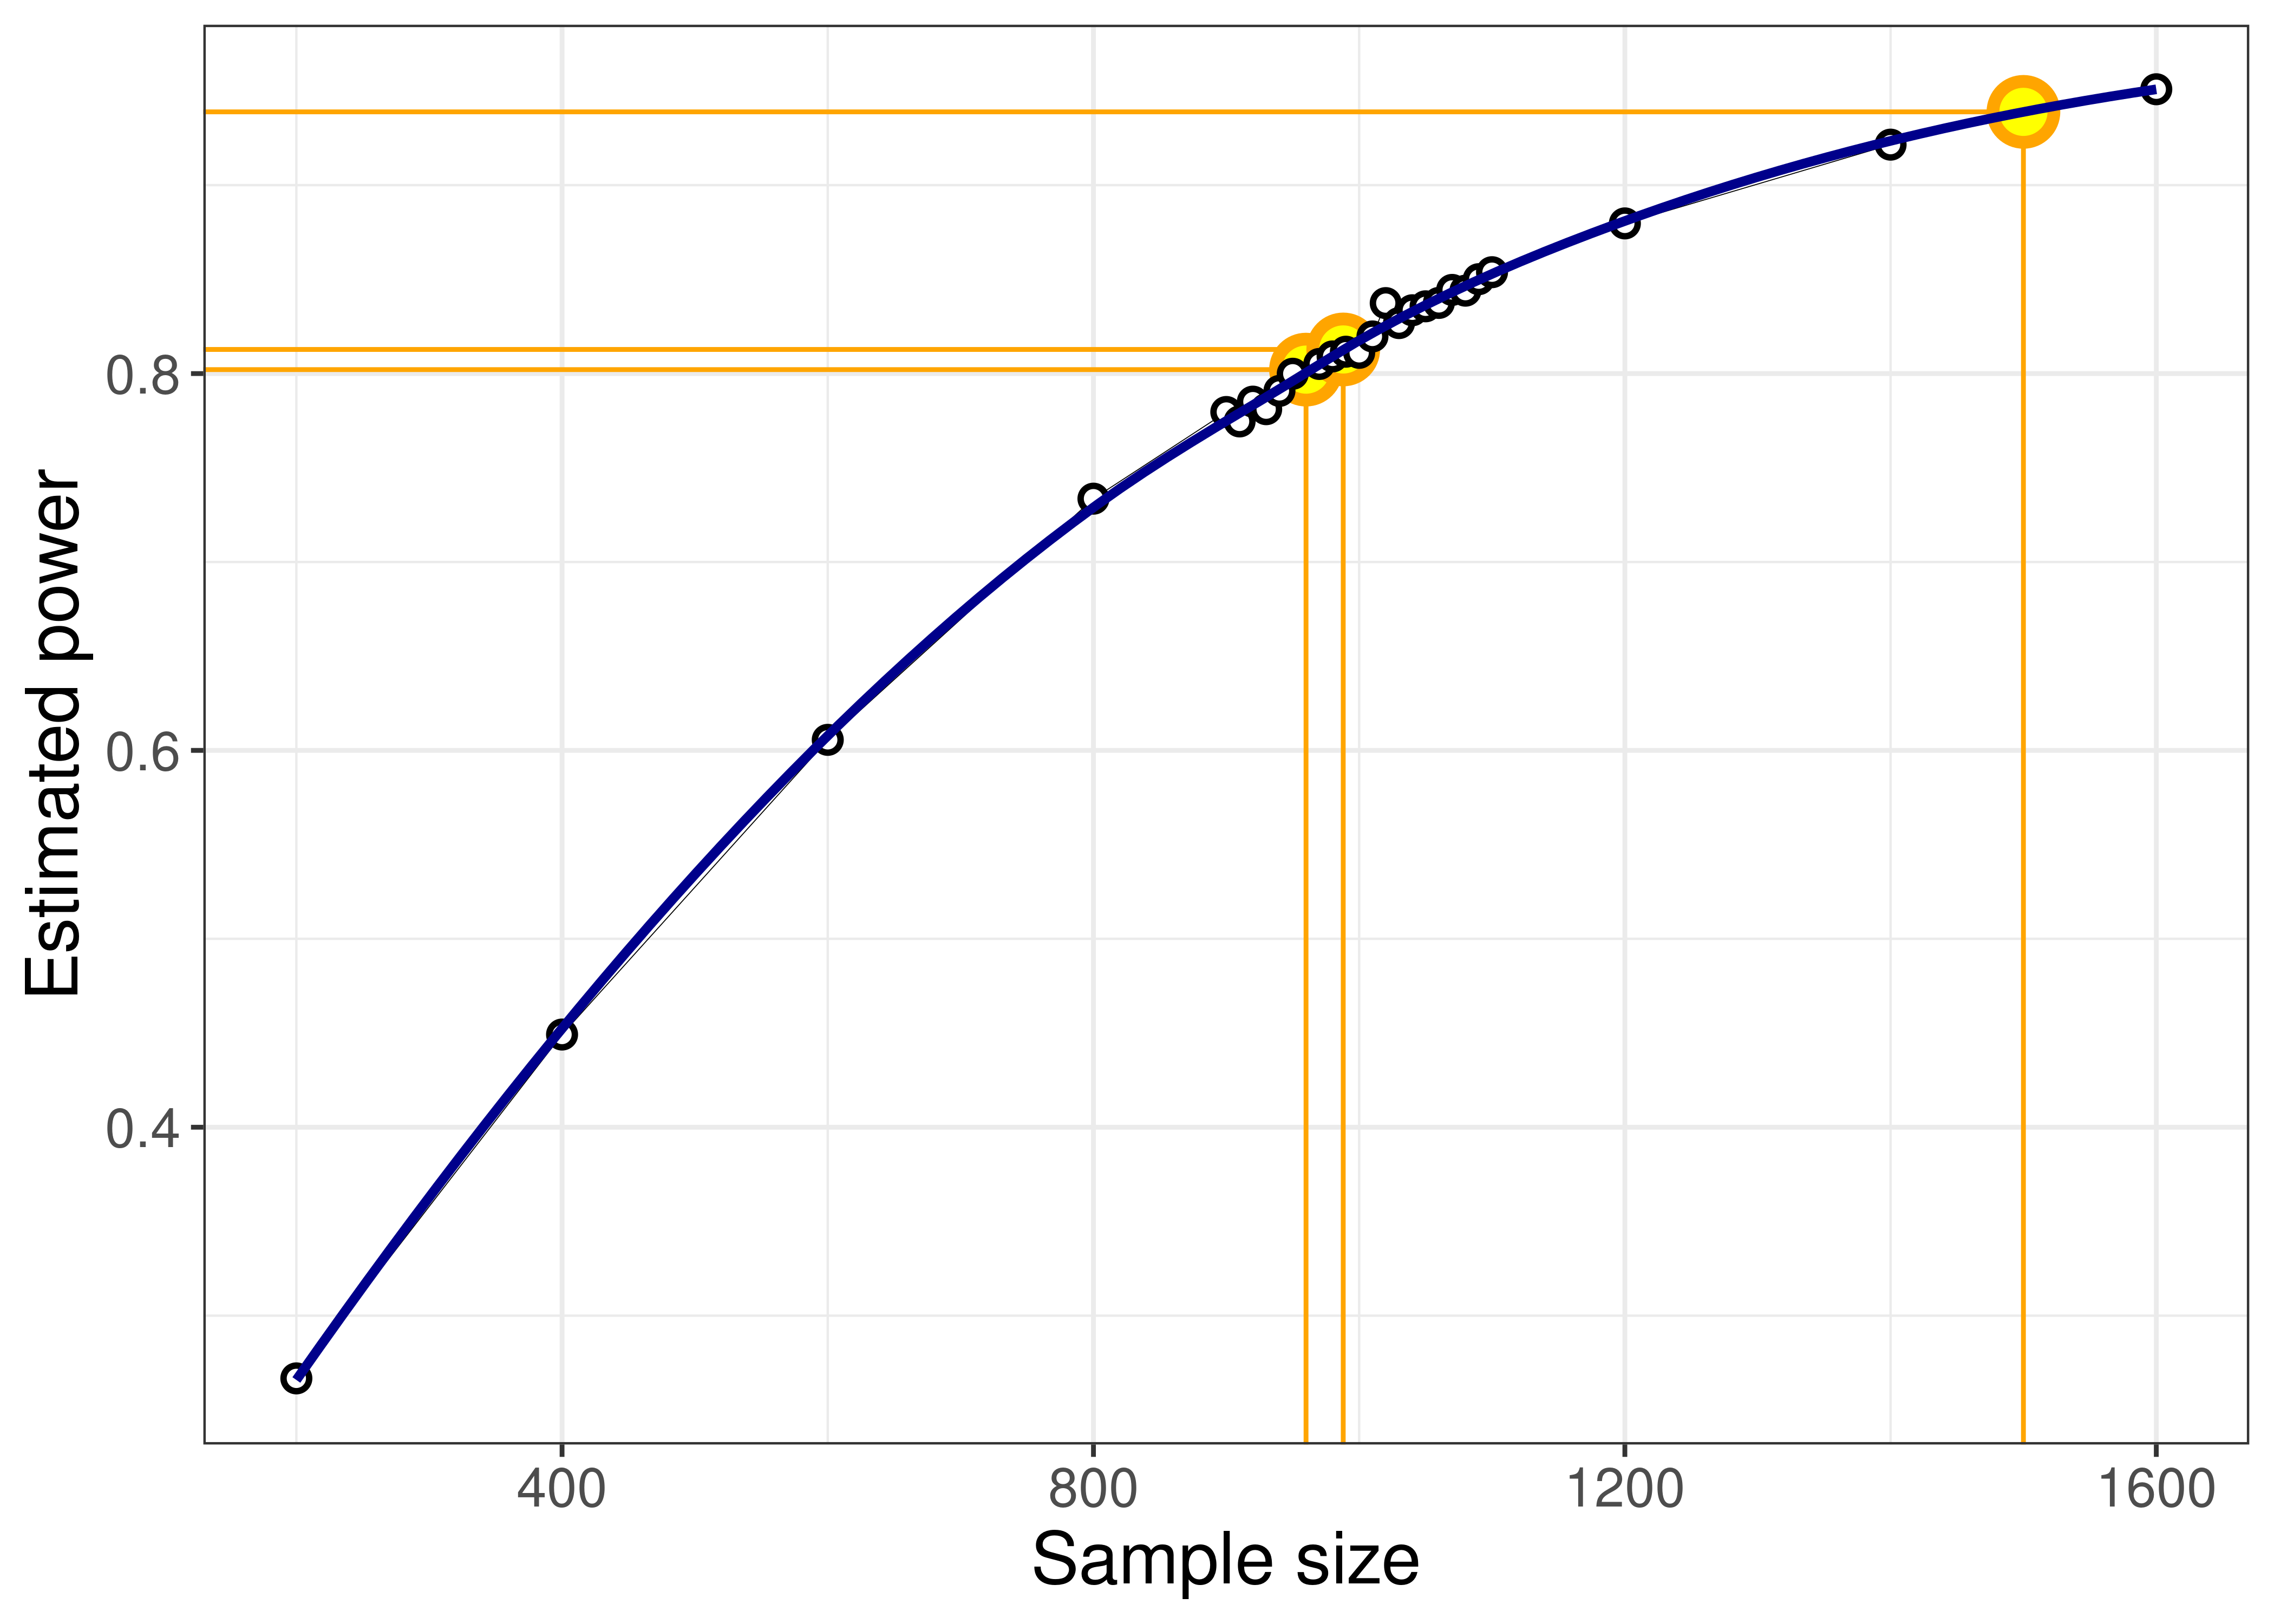
\includegraphics[width=.5\linewidth]{./../analysis/derivatives/power-1.png}
    \mycaption{Sample size and power estimation}{A-priori estimated power for different sample sizes was obtained as the proportion of synthetic data sets in which the null hypothesis of no association between WMH volume and time spent in high-occupancy brain states an be rejected at the $\alpha=0.05$ significance level. Proportions are based on a total of \num{10000} synthetic data sets obtained by bootstrapping the data presented in \citep{Schlemm2022-he}. Highlighted in orange are the smallest sample size ensuring a power of at least \qty{80}{\percent} ($n=960$), the sample size of the pilot data ($n=988$, post-hoc power \qty{81.3}{\percent}), and the expected sample sample size for this replication study ($n=1500$, a-priori power \qty{93.9}{\percent}).}
    \label{fig:power}
\end{figure}

A sample size of \num{960} would have allowed the replication of the reported effect with a power of \qty{80.2}{\percent}.
We had anticipated a sample size of \num{1500}, which would have yielded a power of \qty{93.9}{\percent}.


\subsection{Multiverse analysis}
In both \citep{Schlemm2022-he} and our primary replication analysis, we made certain analytical choices in the operationalization of brain states and ischemic white matter disease, namely the use of the \textit{36p} confound regression strategy, the Schaefer-\num{400} parcellation, and a BIANCA/LOCATE-based WMH segmentation algorithm.
The robustness of the association between WMH burden and time spent in high-occupancy states with regard to other choices was explored in a multiverse analysis \citep{Steegen2016-ze}. Specifically, in an exploratory analysis, we estimated brain states from BOLD time series processed according to a variety of established confound regression strategies and aggregated over different cortical brain parcellations (\Cref{tab:multiverse}, \cite{ciric2018mitigating,Ciric2017-cl}). The extent of cSVD was additionally quantified by the volume of deep and periventricular white matter hyperintensities.

\renewcommand\cellset{\renewcommand\arraystretch{0.5}%
    \setlength\extrarowheight{0pt}}
\begin{table}[bt]
    \begin{threeparttable}
        \begin{subtable}[t]{.75\textwidth}
            \label{tab:parcellations2}
            % Use "S" column identifier to align on decimal point 
            \begin{tabularx}{\textwidth}{l l l}
                \toprule
                \textbf{Name of the atlas}  & \textbf{\#parcels}                                  & \textbf{Reference}          \\
                \midrule
                Desikan--Killiany           & \num{86}                                            & \cite{desikan2006automated} \\
                AAL                         & \num{116}                                           & \cite{tzourio2002automated} \\
                Harvard--Oxford             & \num{112}                                           & \cite{makris2006decreased}  \\
                glasser360                  & \num{360}                                           & \cite{Glasser2016-ia}       \\
                gordon333                   & \num{333}                                           & \cite{Gordon2016-wy}        \\
                power264                    & \num{264}                                           & \cite{Power2011-xf}         \\
                schaefer\{N\}               & \makecell[lt]{\num{100} \\ \num{200}\\ \num{400}}   & \cite{Schaefer2018-bo}      \\
                \bottomrule
            \end{tabularx}
            \begin{tablenotes}
                \item{AAL:} Automatic Anatomical Labelling
            \end{tablenotes}
            \caption{Parcellations}
        \end{subtable}
        \qquad
        \begin{subtable}[t]{.75\textwidth}
            \label{tab:parcellations}
            % Use "S" column identifier to align on decimal point 
            \begin{tabularx}{\textwidth}{l l l}
                \toprule
                \textbf{Design}        & \textbf{Reference}                 \\
                \midrule
                24p                    & \cite{friston1996movement}         \\
                24p + GSR              & \cite{macey2004method}             \\
                36p              & \cite{satterthwaite2013improved}   \\
                36p + spike regression & \cite{cox1996afni}                 \\
                36p + despiking        & \cite{satterthwaite2013improved}   \\
                36p + scrubbing  & \cite{power2014methods}            \\
                aCompCor               & \cite{muschelli2014reduction}      \\
                tCompCor               & \cite{behzadi2007component}        \\
                AROMA                  & \cite{pruim2015ica}                \\
                \bottomrule
            \end{tabularx}
            \begin{tablenotes}
                \item GSR: Global signal regression, AROMA: Automatic Removal of Motion Artifacts
            \end{tablenotes}
            \caption{Confound regression strategies, adapted from \citep{Ciric2017-cl}}
        \end{subtable}
        \makeatletter\def\TPT@hsize{}\makeatletter
    \end{threeparttable}
    \mycaption{Multiverse analysis}{Overview over different brain parcellations and confound regression strategies implemented using xcpEngine \citep{ciric2018mitigating}. A total of $9\times 9=81$ analytical combinations were explored to assess the robustness of our results with respect to these processing choices.}
    \label{tab:multiverse}
\end{table}

For each combination of analytical choice of confound regression strategy, parcellation, and subdivision of white matter lesion load ($9\times9\times3=243$ scenarios in total), we quantified the association between WMH load and average time spent in high-occupancy brain states using odds ratios and \qty{95}{\percent} confidence intervals as described above.

No hypothesis testing was performed for these multiverse analyses. Rather, they serve to inform about the robustness of the outcome of the test of the primary hypothesis.
Any substantial conclusions about the association between the severity of cerebral small vessel pathology and the time spent in high-occupancy brain states were drawn from the primary analysis using pre-specified methodological choices, as stated in the Scientific Question in \Cref{tab:SDT}.

\subsection{Further exploratory analysis}
In previous work, two high-occupancy brain states have been related to the default mode network \citep{Cornblath2020-fu}.
We further explored this relationship by computing, for each individual brain state, the cosine similarity of the positive and negative activations of the cluster’s centroid with a set of a priori defined functional ‘communities’ or networks \citep{Schaefer2018-bo,Yeo2011-qg}.
The results were visualized as spider plots for the Schaefer atlases.

In further exploratory analyses, we describe the associations between brain state dynamics and other measures of cognitive ability such as memory and language.

\subsection{Deviations from preregistration}
For deconfounding and aggregating BOLD data at brain parcellation level, the software xcpEngine was used in version 1.2.3, not 1.2.1, to ensure that that the correct MNI reference template (MNI152NLin2009cAsym) is used for registration of brain atlases. This decision was made before analysing the data.